\section{Algoritmo de Solução para Sistemas Tridiagonais}

\[
 \left[
 \begin{array}{lllllll}
  B_1 & C_1 &        &        &     &        &     \\
  A_2 & B_2 & C_2    &        &     &        &     \\
      & A_3 & B_3    & C_3    &     &        &     \\
      &     & \vdots & \ddots &     &        &     \\
      &     &        & A_i    & B_i & C_i    &     \\
      &     &        &        &     & \ddots &     \\
      &     &        &        &     & A_n    & B_n \\
 \end{array}
 \right]
 \,
 \left[
 \begin{array}{c}
  x_1 \\
  x_2 \\
  x_3 \\
  \vdots \\
  x_i \\
  \vdots \\
  x_n \\
 \end{array}
 \right]
 =
 \left[
 \begin{array}{c}
  D_1 \\
  D_2 \\
  D_3 \\
  \vdots \\
  D_i \\
  \vdots \\
  D_n \\
 \end{array}
 \right]
\]

\esp{
\begin{array}{ll}
 (a) & B'_1 = B_1 \\
     & D'_1 = D_1
\end{array}
}\\

\esp{
\left.
\begin{array}{lll}
 (b) & R    & = A_i\,/\,B'_{i-1} \\
     & B'_i & = B_i - R \, C_{i-1} \\
     & D'_i & = D_i - R \, D'_{i-1}
\end{array}
\right\}
\begin{array}{lll}
 \\
 \mbox{para } i = 2, \, \ldots , \, n \\
 \\
\end{array}
}\\

\esp{
\begin{array}{ll}
 (c) & x_n = D'_n \, / \, B'_n
\end{array}
}\\

\esp{
\begin{array}{ll}
 (d) & x_i = (D'_i - C_i \, x_{i+1}) \, / \, B'_i \qquad i = n-1, \, \ldots , \, 1
\end{array}
}\\

Em \esp{x = 10}

\begin{figure}[htb]
 \centering
 \begin{minipage}[c]{3cm}
    \[
     y'\,(10) = -y_{10} \Rightarrow
    \]
 \end{minipage}\hspace*{2cm}
 \begin{minipage}[c]{5cm}
    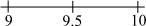
\includegraphics[scale=1.0]{capitulos/capitulo7/figuras/algo_sol_sist_tri1.png}
    %\caption{?}
    \label{fig:algo_sol_sist_tri1}
 \end{minipage}
\end{figure}

\begin{eqnarray}
 && y''\,(10) = \frac{y'\,(10) - y'\,(9.5)}{0.5} \qquad \mbox{(\textit{Backward Difference})} \nonumber \\
 \nonumber \\
 && y'\,(9.5) = \frac{y\,(10) - y\,(9)}{1} \nonumber \\
 \nonumber \\
 && y''\,(10) = \frac{1}{0.5} \, [-y_{10} - y_{10} + y_9]
\end{eqnarray}

Assim

\begin{eqnarray}
 && -2 \, \frac{1}{0.5} \, [-y_{10} - y_{10} + y_9] + y_{10} = e^{-2} \nonumber \\
 \nonumber \\
 && -2 \, y_9 + 4.5 \, y_{10} = 0.5 \, e^{-2}
\end{eqnarray}

Assim

\[
 \left[
 \begin{array}{llllllllll}
  5 & -2 & 0 & 0 & 0 & 0 & 0 & 0 & 0 & 0 \\
  -2 & 5 & -2 & 0 & 0 & 0 & 0 & 0 & 0 & 0 \\
  0 & -2 & 5 & -2 & 0 & 0 & 0 & 0 & 0 & 0 \\
  0 & 0 & -2 & 5 & -2 & 0 & 0 & 0 & 0 & 0 \\
  0 & 0 & 0 & -2 & 5 & -2 & 0 & 0 & 0 & 0 \\
  0 & 0 & 0 & 0 & -2 & 5 & -2 & 0 & 0 & 0 \\
  0 & 0 & 0 & 0 & 0 & -2 & 5 & -2 & 0 & 0 \\
  0 & 0 & 0 & 0 & 0 & 0 & -2 & 5 & -2 & 0 \\
  0 & 0 & 0 & 0 & 0 & 0 & 0 & -2 & 5 & -2 \\
  0 & 0 & 0 & 0 & 0 & 0 & 0 & 0 & -2 & 4.5 \\
 \end{array}
 \right]
 \,
 \left[
 \begin{array}{l}
  y_1 \\
  y_2 \\
  y_3 \\
  y_4 \\
  y_5 \\
  y_6 \\
  y_7 \\
  y_8 \\
  y_9 \\
  y_{10} \\
 \end{array}
 \right]
 =
 \left[
 \begin{array}{l}
  e^{-0.2} + 2 \\
  e^{-0.4} \\
  e^{-0.6} \\
  e^{-0.8} \\
  e^{-1.0} \\
  e^{-1.2} \\
  e^{-1.4} \\
  e^{-1.6} \\
  e^{-1.8} \\
  e^{-2.0} \, \cdot \, 0.5 \\
 \end{array}
 \right]
\]

\begin{example}

Solução pelo método dos elementos finitos.

\begin{enumerate}

\item \textbf{Descrição do problema de valor de contorno}: Encontrar \esp{y\,(x)} tal que a E.D.O. abaixo seja satisfeita em todos os pontos do domínio \esp{D = \{\, x \in R \, | \, 0 \leq x \leq 10 \, \}}

\[
 \left\{
 \begin{array}{l}
  -2 \, y''\,(x) + y\,(x) = e^{-0.2\,x} \\
  \mbox{Condições de contorno} \\
  \qquad y\,(0) = 1 \\
  \qquad y'\,(10) = -y\,(10)
 \end{array}
 \right.
\]

\item \textbf{Discretização do domínio}: \esp{10} elementos conectados aos \esp{11} nós

\begin{figure}[htb]
 \centering
 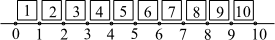
\includegraphics[scale=1.0]{capitulos/capitulo7/figuras/algo_sol_sist_tri2.png}
 \caption{Discretização do domínio}
 \label{fig:algo_sol_sist_tri2}
\end{figure}

\item \textbf{Resíduo}:

\[
 R\,(x) = -2 \, y''\,(x) + y\,(x) - e^{-0.2\,x} = 0
\]

\item \textbf{Formulação Fraca e o Método de Galerkin}

Encontrar \esp{y\,(x)} tal que

\begin{equation}
 \label{cap7:sec2:eq1}
 \int_D \, v\,(x) \, R\,(x) \, dx = 0, \qquad \forall \, v\,(x)
\end{equation}

Considerar \esp{v(x)} no espaço de funções com assentamento local

\begin{figure}[htb]
 \centering
 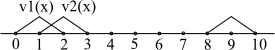
\includegraphics[scale=1.0]{capitulos/capitulo7/figuras/algo_sol_sist_tri3.png}
 \caption{?}
 \label{fig:algo_sol_sist_tri3}
\end{figure}

Assim, \esp{y\,(x)} no intervalo \esp{[1,\,2]} é escrito como uma combinação linear de \esp{v1\,(x)} e \esp{v2\,(x)} ou das restrições \esp{N1\,(x)} e \esp{N2\,(x)} de \esp{v1\,(x)} e \esp{v21\,(x)}, respectivamente, no domínio do elemento \esp{2}.

\[
 y\,(x) = N1\,(x) \, y1 + N2\,(x) \, y2
\]

Também as funções \esp{v\,(x)} no intervalo podem ser escritas como

\[
 v\,(x) = N1\,(x)\,v1 + N2\,(x)\,v2
\]

Substituindo-se o resíduo \esp{R\,(x)} no integrando da equação \ref{cap7:sec2:eq1}, temos

\[
 \int_D \, v\,(x) \, [-2\,y''\,(x) + y\,(x) - e^{-0.2\,x}] \, dx = 0, \qquad \forall \, v\,(x)
\]

\[
 -2 \int_D \, v\,(x) \, y''\,(x) \, dx + \int_D \, v\,(x) \, y\,(x) \, dx - \int_D \, v\,(x) \, e^{-0.2\,x} \, dx = 0, \qquad \forall \, v\,(x)
\]

Integrando-se a primeira integral por partes, temos

\[
 -2 \left[ \left. v\,(x) \, y'\,(x) \right|^{x=10}_{x=0} - \int_D \, v'\,(x) \, y'\,(x) \, dx \right] + \int_D \, v\,(x) \, y\,(x) \, dx - \int_D \, v\,(x) \, e^{-0.2\,x} \, dx = 0, \qquad \forall \, v\,(x)
\]

Utilizando-se a condição de contorno \esp{y'\,(10) = -y\,(10)} e restringindo o espaço de funções \esp{v\,(x)} de forma que \esp{v\,(0) = 0}, temos

\[
 -2 \left[ -v_{10} \, y_{10} - \int_D \, v'\,(x) \, y'\,(x) \, dx \right] + \int_D \, v\,(x) \, y\,(x) \, dx - \int_D \, v\,(x) \, e^{-0.2\,x} \, dx = 0, \qquad \forall \, v\,(x)
\]

Podemos discretizar o domínio \esp{D} em 10 elementos e as integrais podem ser escritas como

\[
 \int_D \, g\,(x) \, dx = \int_0^{10} \, g\,(x) \, dx = \int_0^1 \, g\,(x) \, dx + \int_1^2 \, g\,(x) \, dx + \ldots + \int_9^{10} \, g\,(x) \, dx
\]

Para calcularmos as três integrais restantes, precisamos definir as \esp{N_i\,(x)} e \esp{N_f\,(x)} e calcularmos as derivadas de \esp{v\,(x)} e \esp{y\,(x)}. Assim, com uma parametrização local para cada elemento temos

\begin{figure}[htb]
 \centering
 \begin{minipage}[c]{3cm}
  \[
   \begin{array}{rll}
    N_i\,(\xi) & = & \displaystyle \frac{1 - \xi}{h} \\
    \\
    N_f\,(\xi) & = & \displaystyle \frac{\xi}{h} \\
    \\
    x & = & x_i + \xi \\
    \\
    \xi & = & x - x_i
   \end{array}
  \]
 \end{minipage}\hspace*{2cm}
 \begin{minipage}[c]{5cm}
    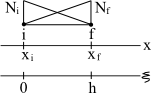
\includegraphics[scale=1.0]{capitulos/capitulo7/figuras/algo_sol_sist_tri4.png}
    %\caption{?}
    \label{fig:algo_sol_sist_tri4}
 \end{minipage}
\end{figure}

\[
 \begin{array}{rll}
  y\,(x) & = & [N_i \, \, N_f] \,
  \left\{
   \begin{array}{c}
    y_i \\
    y_f
   \end{array}
  \right\} \\
  \\
  v\,(x) & = & [N_i \, \, N_f] \,
  \left\{
   \begin{array}{c}
    v_i \\
    v_f
   \end{array}
  \right\} \\
  \\
  y'\,(x) & = & [\displaystyle -\frac{1}{h} \, \, \frac{1}{h}] \,
  \left\{
   \begin{array}{c}
    y_i \\
    y_f
   \end{array}
  \right\} \\
  \\
  v'\,(x) & = & [\displaystyle -\frac{1}{h} \, \, \frac{1}{h}] \,
  \left\{
   \begin{array}{c}
    v_i \\
    v_f
   \end{array}
  \right\}
 \end{array}
\]

\end{enumerate}

\end{example}

Calculando-se as três integrais elemento a elemento, temos

\[
\begin{array}{l}
 \int_{x_i}^{x_f} \, v'\,(x) \, y'\,(x) \, dx = \int_0^h \, v'\,(\xi) \, y'\,(\xi) \, d\xi = [v_i \, \, v_f] \, \int_0^h 
 \,
 \left[
 \begin{array}{rr}
  \displaystyle \frac{1}{h^2} & - \displaystyle \frac{1}{h^2} \\
  \\
  - \displaystyle \frac{1}{h^2} & \displaystyle \frac{1}{h^2} \\
 \end{array}
 \right]
 \,
 d\xi
 \,
 \left\{
  \begin{array}{l}
   y_i \\
   y_f
  \end{array}
 \right\} \\
 \\
 \int_{x_i}^{x_f} \, v\,(x) \, y\,(x) \, dx = \int_0^h \, v\,(\xi) \, y\,(\xi) \, d\xi = [v_i \, \, v_f] \, \int_0^h 
 \,
 \left[
 \begin{array}{ll}
  N_i^2 & N_i\,N_f \\
  N_f\,N_i & N_f^2
 \end{array}
 \right]
 \,
 d\xi
 \,
 \left\{
  \begin{array}{l}
   y_i \\
   y_f
  \end{array}
 \right\} \\
 \\
 \int_{x_i}^{x_f} \, v\,(x) \, e^{-0.2\,x} \, dx = [v_i \, \, v_f] \, \int_0^h 
 \,
 \left[
 \begin{array}{l}
  N_i \, e^{-0.2\,(x_i + \xi)} \\
  N_f \, e^{-0.2\,(x_i + \xi)} \\
 \end{array}
 \right]
 \,
 d\xi
\end{array}
\]
